\documentclass{ximera}

%\usepackage{todonotes}

\newcommand{\todo}{}

\usepackage{esint} % for \oiint
\ifxake%%https://math.meta.stackexchange.com/questions/9973/how-do-you-render-a-closed-surface-double-integral
\renewcommand{\oiint}{{\large\bigcirc}\kern-1.56em\iint}
\fi


\graphicspath{
  {./}
  {ximeraTutorial/}
  {basicPhilosophy/}
  {functionsOfSeveralVariables/}
  {normalVectors/}
  {lagrangeMultipliers/}
  {vectorFields/}
  {greensTheorem/}
  {shapeOfThingsToCome/}
  {dotProducts/}
  {partialDerivativesAndTheGradientVector/}
  {../productAndQuotientRules/exercises/}
  {../normalVectors/exercisesParametricPlots/}
  {../continuityOfFunctionsOfSeveralVariables/exercises/}
  {../partialDerivativesAndTheGradientVector/exercises/}
  {../directionalDerivativeAndChainRule/exercises/}
  {../commonCoordinates/exercisesCylindricalCoordinates/}
  {../commonCoordinates/exercisesSphericalCoordinates/}
  {../greensTheorem/exercisesCurlAndLineIntegrals/}
  {../greensTheorem/exercisesDivergenceAndLineIntegrals/}
  {../shapeOfThingsToCome/exercisesDivergenceTheorem/}
  {../greensTheorem/}
  {../shapeOfThingsToCome/}
  {../separableDifferentialEquations/exercises/}
  {vectorFields/}
}

\newcommand{\mooculus}{\textsf{\textbf{MOOC}\textnormal{\textsf{ULUS}}}}

\usepackage{tkz-euclide}
\usepackage{tikz}
\usepackage{tikz-cd}
\usetikzlibrary{arrows}
\tikzset{>=stealth,commutative diagrams/.cd,
  arrow style=tikz,diagrams={>=stealth}} %% cool arrow head
\tikzset{shorten <>/.style={ shorten >=#1, shorten <=#1 } } %% allows shorter vectors

\usetikzlibrary{backgrounds} %% for boxes around graphs
\usetikzlibrary{shapes,positioning}  %% Clouds and stars
\usetikzlibrary{matrix} %% for matrix
\usepgfplotslibrary{polar} %% for polar plots
\usepgfplotslibrary{fillbetween} %% to shade area between curves in TikZ
%\usetkzobj{all}
\usepackage[makeroom]{cancel} %% for strike outs
%\usepackage{mathtools} %% for pretty underbrace % Breaks Ximera
%\usepackage{multicol}
\usepackage{pgffor} %% required for integral for loops



%% http://tex.stackexchange.com/questions/66490/drawing-a-tikz-arc-specifying-the-center
%% Draws beach ball
\tikzset{pics/carc/.style args={#1:#2:#3}{code={\draw[pic actions] (#1:#3) arc(#1:#2:#3);}}}



\usepackage{array}
\setlength{\extrarowheight}{+.1cm}
\newdimen\digitwidth
\settowidth\digitwidth{9}
\def\divrule#1#2{
\noalign{\moveright#1\digitwidth
\vbox{\hrule width#2\digitwidth}}}




% \newcommand{\RR}{\mathbb R}
% \newcommand{\R}{\mathbb R}
% \newcommand{\N}{\mathbb N}
% \newcommand{\Z}{\mathbb Z}

\newcommand{\sagemath}{\textsf{SageMath}}


%\renewcommand{\d}{\,d\!}
%\renewcommand{\d}{\mathop{}\!d}
%\newcommand{\dd}[2][]{\frac{\d #1}{\d #2}}
%\newcommand{\pp}[2][]{\frac{\partial #1}{\partial #2}}
% \renewcommand{\l}{\ell}
%\newcommand{\ddx}{\frac{d}{\d x}}

% \newcommand{\zeroOverZero}{\ensuremath{\boldsymbol{\tfrac{0}{0}}}}
%\newcommand{\inftyOverInfty}{\ensuremath{\boldsymbol{\tfrac{\infty}{\infty}}}}
%\newcommand{\zeroOverInfty}{\ensuremath{\boldsymbol{\tfrac{0}{\infty}}}}
%\newcommand{\zeroTimesInfty}{\ensuremath{\small\boldsymbol{0\cdot \infty}}}
%\newcommand{\inftyMinusInfty}{\ensuremath{\small\boldsymbol{\infty - \infty}}}
%\newcommand{\oneToInfty}{\ensuremath{\boldsymbol{1^\infty}}}
%\newcommand{\zeroToZero}{\ensuremath{\boldsymbol{0^0}}}
%\newcommand{\inftyToZero}{\ensuremath{\boldsymbol{\infty^0}}}



% \newcommand{\numOverZero}{\ensuremath{\boldsymbol{\tfrac{\#}{0}}}}
% \newcommand{\dfn}{\textbf}
% \newcommand{\unit}{\,\mathrm}
% \newcommand{\unit}{\mathop{}\!\mathrm}
% \newcommand{\eval}[1]{\bigg[ #1 \bigg]}
% \newcommand{\seq}[1]{\left( #1 \right)}
% \renewcommand{\epsilon}{\varepsilon}
% \renewcommand{\phi}{\varphi}


% \renewcommand{\iff}{\Leftrightarrow}

% \DeclareMathOperator{\arccot}{arccot}
% \DeclareMathOperator{\arcsec}{arcsec}
% \DeclareMathOperator{\arccsc}{arccsc}
% \DeclareMathOperator{\si}{Si}
% \DeclareMathOperator{\scal}{scal}
% \DeclareMathOperator{\sign}{sign}


%% \newcommand{\tightoverset}[2]{% for arrow vec
%%   \mathop{#2}\limits^{\vbox to -.5ex{\kern-0.75ex\hbox{$#1$}\vss}}}
% \newcommand{\arrowvec}[1]{{\overset{\rightharpoonup}{#1}}}
% \renewcommand{\vec}[1]{\arrowvec{\mathbf{#1}}}
% \renewcommand{\vec}[1]{{\overset{\boldsymbol{\rightharpoonup}}{\mathbf{#1}}}}

% \newcommand{\point}[1]{\left(#1\right)} %this allows \vector{ to be changed to \vector{ with a quick find and replace
% \newcommand{\pt}[1]{\mathbf{#1}} %this allows \vec{ to be changed to \vec{ with a quick find and replace
% \newcommand{\Lim}[2]{\lim_{\point{#1} \to \point{#2}}} %Bart, I changed this to point since I want to use it.  It runs through both of the exercise and exerciseE files in limits section, which is why it was in each document to start with.

% \DeclareMathOperator{\proj}{\mathbf{proj}}
% \newcommand{\veci}{{\boldsymbol{\hat{\imath}}}}
% \newcommand{\vecj}{{\boldsymbol{\hat{\jmath}}}}
% \newcommand{\veck}{{\boldsymbol{\hat{k}}}}
% \newcommand{\vecl}{\vec{\boldsymbol{\l}}}
% \newcommand{\uvec}[1]{\mathbf{\hat{#1}}}
% \newcommand{\utan}{\mathbf{\hat{t}}}
% \newcommand{\unormal}{\mathbf{\hat{n}}}
% \newcommand{\ubinormal}{\mathbf{\hat{b}}}

% \newcommand{\dotp}{\bullet}
% \newcommand{\cross}{\boldsymbol\times}
% \newcommand{\grad}{\boldsymbol\nabla}
% \newcommand{\divergence}{\grad\dotp}
% \newcommand{\curl}{\grad\cross}
%\DeclareMathOperator{\divergence}{divergence}
%\DeclareMathOperator{\curl}[1]{\grad\cross #1}
% \newcommand{\lto}{\mathop{\longrightarrow\,}\limits}

% \renewcommand{\bar}{\overline}

\colorlet{textColor}{black}
\colorlet{background}{white}
\colorlet{penColor}{blue!50!black} % Color of a curve in a plot
\colorlet{penColor2}{red!50!black}% Color of a curve in a plot
\colorlet{penColor3}{red!50!blue} % Color of a curve in a plot
\colorlet{penColor4}{green!50!black} % Color of a curve in a plot
\colorlet{penColor5}{orange!80!black} % Color of a curve in a plot
\colorlet{penColor6}{yellow!70!black} % Color of a curve in a plot
\colorlet{fill1}{penColor!20} % Color of fill in a plot
\colorlet{fill2}{penColor2!20} % Color of fill in a plot
\colorlet{fillp}{fill1} % Color of positive area
\colorlet{filln}{penColor2!20} % Color of negative area
\colorlet{fill3}{penColor3!20} % Fill
\colorlet{fill4}{penColor4!20} % Fill
\colorlet{fill5}{penColor5!20} % Fill
\colorlet{gridColor}{gray!50} % Color of grid in a plot

\newcommand{\surfaceColor}{violet}
\newcommand{\surfaceColorTwo}{redyellow}
\newcommand{\sliceColor}{greenyellow}




\pgfmathdeclarefunction{gauss}{2}{% gives gaussian
  \pgfmathparse{1/(#2*sqrt(2*pi))*exp(-((x-#1)^2)/(2*#2^2))}%
}


%%%%%%%%%%%%%
%% Vectors
%%%%%%%%%%%%%

%% Simple horiz vectors
\renewcommand{\vector}[1]{\left\langle #1\right\rangle}


%% %% Complex Horiz Vectors with angle brackets
%% \makeatletter
%% \renewcommand{\vector}[2][ , ]{\left\langle%
%%   \def\nextitem{\def\nextitem{#1}}%
%%   \@for \el:=#2\do{\nextitem\el}\right\rangle%
%% }
%% \makeatother

%% %% Vertical Vectors
%% \def\vector#1{\begin{bmatrix}\vecListA#1,,\end{bmatrix}}
%% \def\vecListA#1,{\if,#1,\else #1\cr \expandafter \vecListA \fi}

%%%%%%%%%%%%%
%% End of vectors
%%%%%%%%%%%%%

%\newcommand{\fullwidth}{}
%\newcommand{\normalwidth}{}



%% makes a snazzy t-chart for evaluating functions
%\newenvironment{tchart}{\rowcolors{2}{}{background!90!textColor}\array}{\endarray}

%%This is to help with formatting on future title pages.
\newenvironment{sectionOutcomes}{}{}



%% Flowchart stuff
%\tikzstyle{startstop} = [rectangle, rounded corners, minimum width=3cm, minimum height=1cm,text centered, draw=black]
%\tikzstyle{question} = [rectangle, minimum width=3cm, minimum height=1cm, text centered, draw=black]
%\tikzstyle{decision} = [trapezium, trapezium left angle=70, trapezium right angle=110, minimum width=3cm, minimum height=1cm, text centered, draw=black]
%\tikzstyle{question} = [rectangle, rounded corners, minimum width=3cm, minimum height=1cm,text centered, draw=black]
%\tikzstyle{process} = [rectangle, minimum width=3cm, minimum height=1cm, text centered, draw=black]
%\tikzstyle{decision} = [trapezium, trapezium left angle=70, trapezium right angle=110, minimum width=3cm, minimum height=1cm, text centered, draw=black]


\title{Assemble}

\begin{document}

\begin{abstract}
putting functions together
\end{abstract}
\maketitle





The elementary functions are too nice.

They don't do anything interesting.

However, the world of functions is crazy.  Functions behave in very unexpected ways, which we'll never see if we stick to the elementary functions.

For a meaningful investigation of functions, we need to explore other types of functions.

We can create new functions from the elementary functions by creating sums, differences, products, and quotients.


We can create new functions from the elementary functions by creating piecewise defined functions.


We can create new functions from the elementary functions by composing them. 




\begin{template} \textbf{\textcolor{blue!55!black}{Composition}}  \\


Let $f$ be a function with domain $D_f$.


Let $g$ be a function with domain $D_g$.




Then the \textbf{\textcolor{green!50!black}{composition of f and g, $f \circ g$,}} is defined as

\[
(f \circ g)(x) = f(g(x))
\] 


The value of $g$ becomes a domain number for $f$.


The composition is defined on a subset of the domain of $g$.  The composition is defined at those numbers in the domain of $g$ where the value of $g$ is in the domain of $f$.




\end{template}







\begin{example}


Let $f(x) = 3 - x$ with its natural domain.


Let $g(y) = \ln(y)$ with its natural domain.


Defines $H = f \circ g$ with its natural domain.



\begin{explanation}


$H(t) = (f \circ g)(t) = f(g(t))$


The domain of $H = f \circ g$ is a subset of the domain of $g$, which is $(0, \infty)$.  

We can only use those numbers where $ln(t)$ is in the domain of $f$.  However, the domain of $f$ is all real numbers.  So, we can use everything from the domain of $g$.

The induced domain of $H = f \circ g$ is the domain of $g$, which is $(0, \infty)$. 




\end{explanation}







\begin{explanation}


$K(r) = (g \circ f)(r) = g(f(r))$


The domain of $K = g \circ f$ is a subset of the domain of $f$, which is $(-\infty, \infty)$.  

We can only use those numbers where $f(r)$ is in the domain of $g$.  The domain of $g$ is $(0, \infty)$.  

Therefore, we need $f(x) = 3 - x > 0$.  Or, $x < 3$.

The induced domain of $K = g \circ f$ is $(-\infty, 3)$. 

These are the numbers in the domain of $f$ where the value of $f$ is inside the domain of $g$.


\end{explanation}




\end{example}


An \textbf{induced} domain is a domain that is force to happen due to given restrictions. \\







\begin{example}



Let $T(x) = (3-x)(x-5)$ with its natural domain.


Let $p(t) = \frac{1}{t}$ with its natural domain.


Defines $Y = T \circ p$ with its natural domain.



\begin{question}

Evaluate


\[
(T \circ p)\left( \frac{1}{2} \right) = \answer{-3}
\]



\end{question}






\begin{question}

Evaluate


\[
(p \circ T)\left( \frac{1}{2} \right) = \answer{-\frac{4}{45}}
\]



\end{question}





\begin{question}

What is the induced domain of $(T \circ p)$?


\[
\left( \answer{-\infty}, \answer{0}  \right) \cup \left( \answer{0}, \answer{\infty}  \right)
\]



\end{question}








\begin{question}

What is the induced domain of $(p \circ T)$?


\[
\left( \answer{-\infty}, \answer{3}  \right) \cup \left( \answer{3}, \answer{5}  \right)  \cup \left( \answer{5}, \answer{\infty}  \right)
\]



\end{question}







\end{example}



















































Let $Out(x) = 2|x-3|+1$ with its natural or implied domain. \\

Let $In(t) = -(t-1)^2 + 5$ with its natural or implied domain. \\









Graph of $y = Out(x) =2|x-3|+1$

\begin{image}
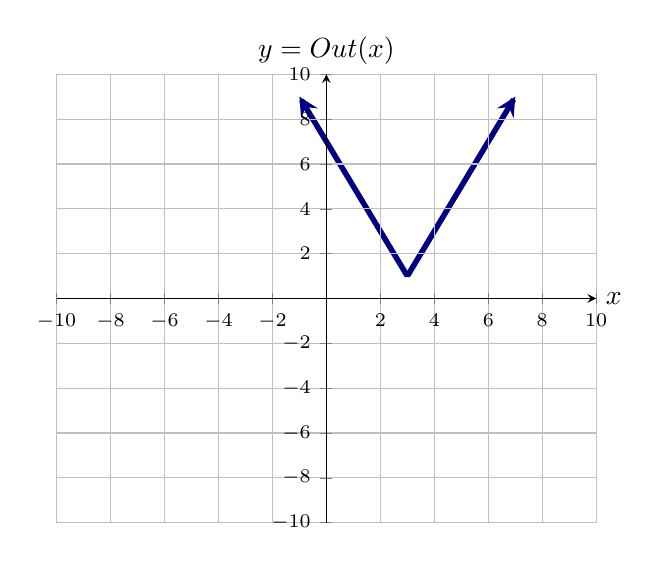
\begin{tikzpicture}
  \begin{axis}[
            domain=-10:10, ymax=10, xmax=10, ymin=-10, xmin=-10,
            axis lines =center, xlabel=$x$, ylabel={$y=Out(x)$}, grid = major,
            ytick={-10,-8,-6,-4,-2,2,4,6,8,10},
            xtick={-10,-8,-6,-4,-2,2,4,6,8,10},
            yticklabels={$-10$,$-8$,$-6$,$-4$,$-2$,$2$,$4$,$6$,$8$,$10$}, 
            xticklabels={$-10$,$-8$,$-6$,$-4$,$-2$,$2$,$4$,$6$,$8$,$10$},
            ticklabel style={font=\scriptsize},
            every axis y label/.style={at=(current axis.above origin),anchor=south},
            every axis x label/.style={at=(current axis.right of origin),anchor=west},
            axis on top
          ]
          
          %\addplot [line width=2, penColor2, smooth,samples=100,domain=(-6:2)] {-2*x-3};
			\addplot [line width=2, penColor, smooth,samples=100,domain=(-1:7),<->] {2*abs(x-3)+1};

          %\addplot[color=penColor,fill=penColor2,only marks,mark=*] coordinates{(-6,9)};
          %\addplot[color=penColor,fill=penColor2,only marks,mark=*] coordinates{(2,-7)};



           

  \end{axis}
\end{tikzpicture}
\end{image}
The natural domain of $Out$ is $\mathbb{R}$. \\

The graph of $Out$ has a ``V''-shape, opening up, with a corner at $(3,1)$. \\
This illustrates that $Out$ decreases on $(-\infty, 3]$ and increases on $[3, \infty)$.  $Out$ has a minimum value of $1$, which occurs at $3$. \\

If we think of tracing the domain from left to right on the graph, the corresponding values of $Out$ decrease from $\infty$ down to $1$, then reverse direction and increase from $1$ back to $\infty$. \\



The only values that can come out of the composition, $Out \circ In$, are the values of $Out$. Therefore, the values of $Out \circ In$ are inside the interval $[1, \infty)$.  



Graph of $z = In(t) = -(t-1)^2 + 5$





\begin{image}
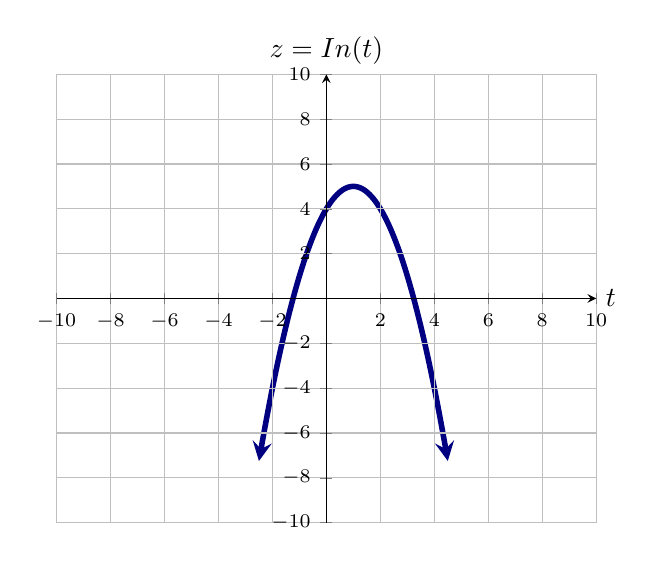
\begin{tikzpicture}
  \begin{axis}[
            domain=-10:10, ymax=10, xmax=10, ymin=-10, xmin=-10,
            axis lines =center, xlabel=$t$, ylabel={$z=In(t)$}, grid = major,
            ytick={-10,-8,-6,-4,-2,2,4,6,8,10},
            xtick={-10,-8,-6,-4,-2,2,4,6,8,10},
            yticklabels={$-10$,$-8$,$-6$,$-4$,$-2$,$2$,$4$,$6$,$8$,$10$}, 
            xticklabels={$-10$,$-8$,$-6$,$-4$,$-2$,$2$,$4$,$6$,$8$,$10$},
            ticklabel style={font=\scriptsize},
            every axis y label/.style={at=(current axis.above origin),anchor=south},
            every axis x label/.style={at=(current axis.right of origin),anchor=west},
            axis on top
          ]
          
          %\addplot [line width=2, penColor2, smooth,samples=100,domain=(-6:2)] {-2*x-3};
			\addplot [line width=2, penColor, smooth,samples=100,domain=(-2.5:4.5),<->] {-(x-1)^2 + 5)};

          %\addplot[color=penColor,fill=penColor2,only marks,mark=*] coordinates{(-6,9)};
          %\addplot[color=penColor,fill=penColor2,only marks,mark=*] coordinates{(2,-7)};



           

  \end{axis}
\end{tikzpicture}
\end{image}
The natural domain of $In$ is $\mathbb{R}$. \\


Since $In$ is a quadratic function, its graph has the shape of a parabola, opening down.  $In$ increases on $(-\infty, 1]$ and decreases on $[1, \infty)$. $In$ has a maximum value of $5$, which occurs at $1$. \\

If we think of tracing the domain from left to right on the graph, the values of $In$ increase from $-\infty$ up to $5$, then reverse direction and decrease from $5$ back to $-\infty$.


The output from the function $In$ will become the input to $Out$.  Therefore, in the composition, the new input to $Out$ will be the interval $(-\infty, 5]$, which is the output of $In$. This interval is traced twice: the values going into $Out$ will begin at $-\infty$, go up to $5$, then turn around and go back down to $-\infty$. The values of $Out$ will similarly repeat themselves in reverse.\\






\textbf{\textcolor{purple!85!blue}{Now to examine the composition:}} \\



\textbf{\textcolor{blue!75!black}{$\blacktriangleright$}}   First, the inside function: $In(t) = -(t-1)^2 + 5$ \\

The natural domain of $In(t)$ is the whole real line. As we move from left to right along the real line, the domain numbers increase from $-\infty$ to $\infty$.

The corresponding movement in the range has the function values increasing from $-\infty$ to $5$.  The maximum function value $5$ occurs at $1$ in the domain.  As we keep moving beyond $1$ in the domain, the corresponding movement in the range is for the function values to decrease from $5$ to $-\infty$.


This path in the range of $In(t)$ becomes the path in the domain of $Out(x)$. \\













\begin{image}
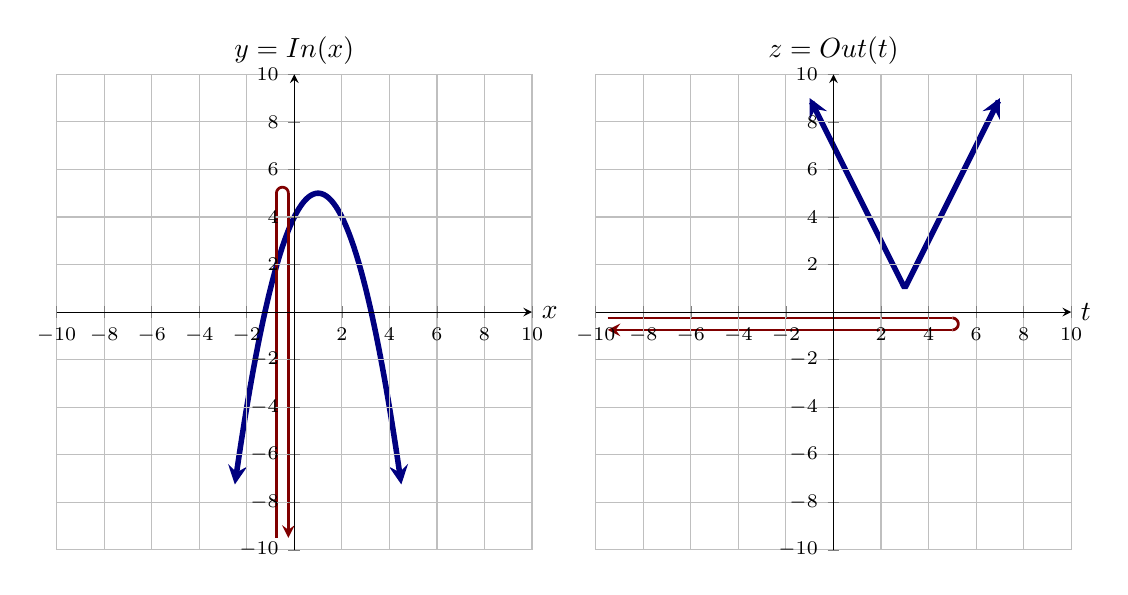
\begin{tikzpicture}
    \begin{axis}[name = sinax, domain=-10:10, ymax=10, xmax=10, ymin=-10, xmin=-10, width=3in, height=3in,
                  axis lines =center, xlabel=$x$, ylabel={$y=In(x)$}, grid = major,
                  ytick={-10,-8,-6,-4,-2,2,4,6,8,10},
                  xtick={-10,-8,-6,-4,-2,2,4,6,8,10},
                  yticklabels={$-10$,$-8$,$-6$,$-4$,$-2$,$2$,$4$,$6$,$8$,$10$}, 
                  xticklabels={$-10$,$-8$,$-6$,$-4$,$-2$,$2$,$4$,$6$,$8$,$10$},
                  ticklabel style={font=\scriptsize},
                  every axis y label/.style={at=(current axis.above origin),anchor=south},
                  every axis x label/.style={at=(current axis.right of origin),anchor=west},
                  axis on top]
        \addplot [line width=2, penColor, smooth,samples=100,domain=(-2.5:4.5),<->] {-(x-1)^2 + 5)};

        \addplot [line width=1, penColor2, smooth, domain=(-9.5:5)] ({-0.75},{x});
        \addplot [line width=1, penColor2, smooth, domain=(-9.5:5),<-] ({-0.25},{x});
        \addplot [line width=1, penColor2, smooth, domain=(0:3.14)] ({0.25*cos(deg(x))-0.5},{0.25*sin(deg(x))+5});

    \end{axis}
    \begin{axis}[at={(sinax.outer east)},anchor=outer west, domain=-10:10, ymax=10, xmax=10, ymin=-10, xmin=-10, 
                  width=3in, height=3in,
                  axis lines =center, xlabel=$t$, ylabel={$z=Out(t)$}, grid = major,
                  ytick={-10,-8,-6,-4,-2,2,4,6,8,10},
                  xtick={-10,-8,-6,-4,-2,2,4,6,8,10},
                  yticklabels={$-10$,$-8$,$-6$,$-4$,$-2$,$2$,$4$,$6$,$8$,$10$}, 
                  xticklabels={$-10$,$-8$,$-6$,$-4$,$-2$,$2$,$4$,$6$,$8$,$10$},
                  ticklabel style={font=\scriptsize},
                  every axis y label/.style={at=(current axis.above origin),anchor=south},
                  every axis x label/.style={at=(current axis.right of origin),anchor=west},
                  axis on top]
        \addplot [line width=2, penColor, smooth,samples=100,domain=(-1:7),<->] {2*abs(x-3)+1};

        \addplot [line width=1, penColor2, smooth, domain=(-9.5:5)] ({x},{-0.25});
        \addplot [line width=1, penColor2, smooth, domain=(-9.5:5),<-] ({x},{-0.75});
        \addplot [line width=1, penColor2, smooth, domain=(-1.57:1.57)] ({0.25*cos(deg(x))+5},{0.25*sin(deg(x))-0.5});

    \end{axis}


\end{tikzpicture}
\end{image}



















\textbf{\textcolor{blue!75!black}{$\blacktriangleright$}}  Movement inside the domain of $Out(x)$.\\



Inside the natural domain of $Out(x) =2|x-3|+1$, the domain numbers will increase from $-\infty$ to $5$.  Then they will decrease from $5$ back down to $-\infty$. \\

Following our graph of $Out(x)$, we will move from the far left toward the right until we reach $5$.  Then we will turn around and move toward the left.\\



\textbf{\textcolor{blue!75!black}{$\blacktriangleright$}}  Put those together. \\



We have the input to $Out$ moving from $-\infty$ up to $5$ and then back down to $-\infty$.  What are the corresponding function values for $Out$?





\begin{itemize}

\item As the domain numbers move through $(-\infty, 5]$, the values of $Out$ decrease from $\infty$ to $1$ and then increase from $1$ to $5$.  In the graph, we can see this switch as a corner in the graph. The graph comes down to the right, hits the corner, then moves back up to the right.





\begin{image}
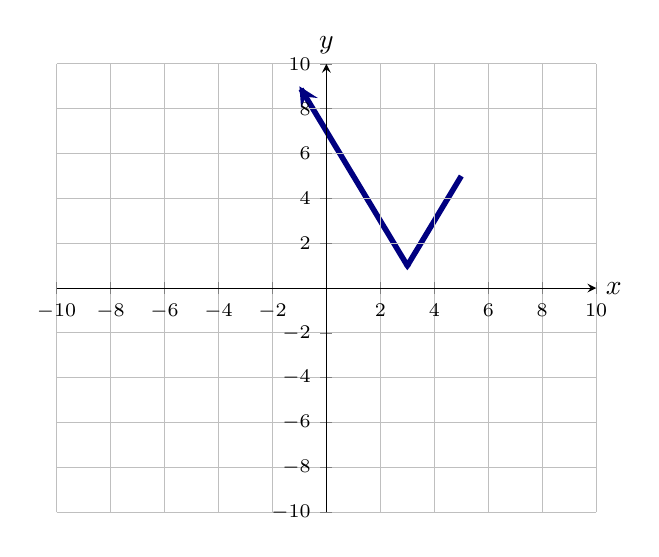
\begin{tikzpicture}
  \begin{axis}[
            domain=-10:10, ymax=10, xmax=10, ymin=-10, xmin=-10,
            axis lines =center, xlabel=$x$, ylabel=$y$, grid = major,
            ytick={-10,-8,-6,-4,-2,2,4,6,8,10},
            xtick={-10,-8,-6,-4,-2,2,4,6,8,10},
            yticklabels={$-10$,$-8$,$-6$,$-4$,$-2$,$2$,$4$,$6$,$8$,$10$}, 
            xticklabels={$-10$,$-8$,$-6$,$-4$,$-2$,$2$,$4$,$6$,$8$,$10$},
            ticklabel style={font=\scriptsize},
            every axis y label/.style={at=(current axis.above origin),anchor=south},
            every axis x label/.style={at=(current axis.right of origin),anchor=west},
            axis on top
          ]
          
          %\addplot [line width=2, penColor2, smooth,samples=100,domain=(-6:2)] {-2*x-3};
      \addplot [line width=2, penColor, smooth,samples=100,domain=(-1:5),<-] {2*abs(x-3)+1};
      

          %\addplot[color=penColor,fill=penColor2,only marks,mark=*] coordinates{(-6,9)};
          %\addplot[color=penColor,fill=penColor2,only marks,mark=*] coordinates{(2,-7)};



           

  \end{axis}
\end{tikzpicture}
\end{image}




So, we really should view $(-\infty, 5]$  as  $(-\infty, 3] \cup [3,5]$ and highlight the change in behavior.







\begin{image}
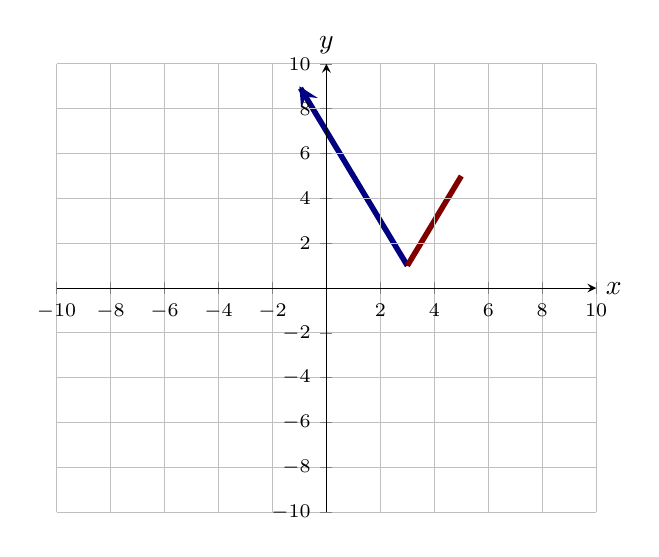
\begin{tikzpicture}
  \begin{axis}[
            domain=-10:10, ymax=10, xmax=10, ymin=-10, xmin=-10,
            axis lines =center, xlabel=$x$, ylabel=$y$, grid = major,
            ytick={-10,-8,-6,-4,-2,2,4,6,8,10},
            xtick={-10,-8,-6,-4,-2,2,4,6,8,10},
            yticklabels={$-10$,$-8$,$-6$,$-4$,$-2$,$2$,$4$,$6$,$8$,$10$}, 
            xticklabels={$-10$,$-8$,$-6$,$-4$,$-2$,$2$,$4$,$6$,$8$,$10$},
            ticklabel style={font=\scriptsize},
            every axis y label/.style={at=(current axis.above origin),anchor=south},
            every axis x label/.style={at=(current axis.right of origin),anchor=west},
            axis on top
          ]
          
          %\addplot [line width=2, penColor2, smooth,samples=100,domain=(-6:2)] {-2*x-3};
      \addplot [line width=2, penColor, smooth,samples=100,domain=(-1:3),<-] {2*abs(x-3)+1};
      \addplot [line width=2, penColor2, smooth,samples=100,domain=(3:5)] {2*abs(x-3)+1};

          %\addplot[color=penColor,fill=penColor2,only marks,mark=*] coordinates{(-6,9)};
          %\addplot[color=penColor,fill=penColor2,only marks,mark=*] coordinates{(2,-7)};



           

  \end{axis}
\end{tikzpicture}
\end{image}




	\begin{itemize}[label=$\star$]
		\item On $(-\infty, 3]$, $Out$ decreases from $\infty$ to $1$.

		\item On $[3,5]$, $Out$ increases from $1$ to $5$

	\end{itemize}



That was on our first pass through $(-\infty, 5]$. \\



The input to $Out$ continues beginning at $5$ and moving towards $-\infty$.  \\

As the overall domain to the whole compostion continues to cover $[5, \infty)$, The function $In$ reverses this interval and sends the reversed interval into $Out$. As the overall composition domain continues to move through $[5, \infty)$, the input to $Out$ traces backwards from $5$ to $-\infty$.  The overall composition graph keeps moving to the right, but it is retracing the left side in reverse, mirroring it.




\item Moving backwards through $(-\infty, 5]$, The values of $Out$ first decrease from $5$ to $1$, arriving again at the corner that occurs at $3$.  Again, we really should look at $(-\infty, 5]$  as  $(-\infty, 3] \cup [3,5]$.

	\begin{itemize}
		\item As the domain moves from $5$ to $3$, $Out$ decreases from $5$ to $1$.

		\item As the domain moves from $3$ to $-\infty$, $Out$ increases from $1$ to $\infty$.

	\end{itemize}

\end{itemize}

Since we reverse our travelling direction inside the domain, we hit the corner twice.  Plus, right at our reversal, we will create a hill in the graph made by our own retracing of the domain steps.






\begin{image}
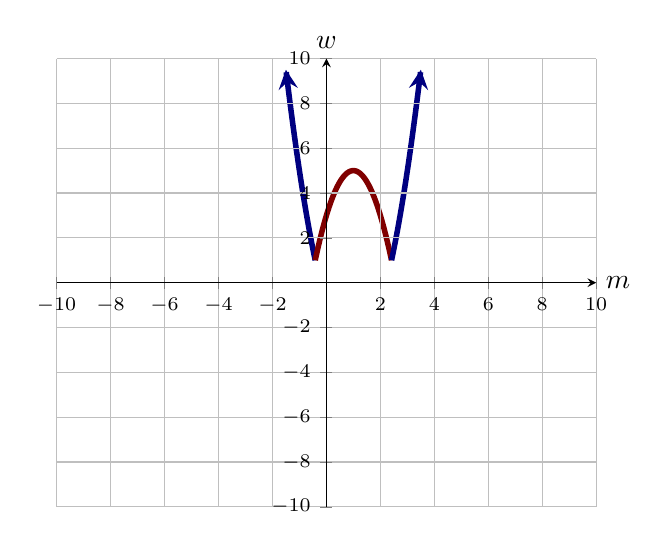
\begin{tikzpicture}
  \begin{axis}[
            domain=-10:10, ymax=10, xmax=10, ymin=-10, xmin=-10,
            axis lines =center, xlabel=$m$, ylabel=$w$, grid = major,
            ytick={-10,-8,-6,-4,-2,2,4,6,8,10},
            xtick={-10,-8,-6,-4,-2,2,4,6,8,10},
            yticklabels={$-10$,$-8$,$-6$,$-4$,$-2$,$2$,$4$,$6$,$8$,$10$}, 
            xticklabels={$-10$,$-8$,$-6$,$-4$,$-2$,$2$,$4$,$6$,$8$,$10$},
            ticklabel style={font=\scriptsize},
            every axis y label/.style={at=(current axis.above origin),anchor=south},
            every axis x label/.style={at=(current axis.right of origin),anchor=west},
            axis on top
          ]
            \addplot [line width=2, penColor, smooth,samples=100,domain=(-1.5:-0.414),<-] {2*abs(-(x-1)^2 + 2)+1};
            \addplot [line width=2, penColor2, smooth,samples=100,domain=(-0.414:2.414)] {2*abs(-(x-1)^2 + 2)+1};
            \addplot [line width=2, penColor, smooth,samples=100,domain=(2.414:3.5),->] {2*abs(-(x-1)^2 + 2)+1};

  \end{axis}
\end{tikzpicture}
\end{image}














\textbf{\textcolor{blue!55!black}{All together now...}}   \\


Graph of $w = Out(In(m)) =2 \, |(-(m-1)^2 + 5)-3|+1 = 2 \, |-(m-1)^2 + 2| + 1$







\begin{image}
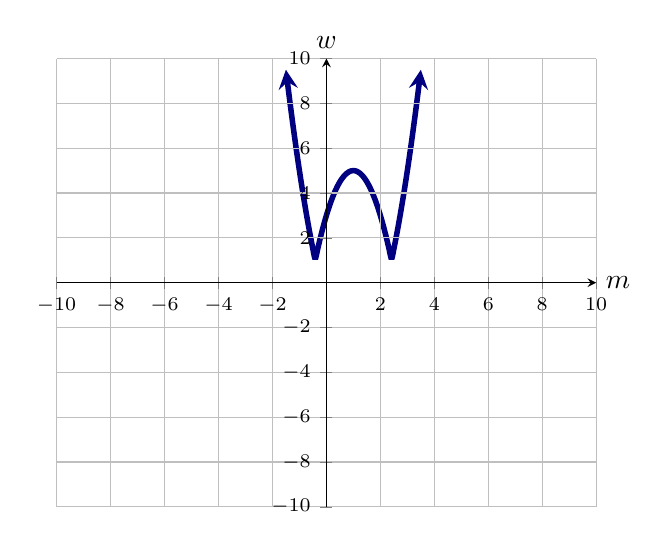
\begin{tikzpicture}
  \begin{axis}[
            domain=-10:10, ymax=10, xmax=10, ymin=-10, xmin=-10,
            axis lines =center, xlabel=$m$, ylabel=$w$, grid = major,
            ytick={-10,-8,-6,-4,-2,2,4,6,8,10},
            xtick={-10,-8,-6,-4,-2,2,4,6,8,10},
            yticklabels={$-10$,$-8$,$-6$,$-4$,$-2$,$2$,$4$,$6$,$8$,$10$}, 
            xticklabels={$-10$,$-8$,$-6$,$-4$,$-2$,$2$,$4$,$6$,$8$,$10$},
            ticklabel style={font=\scriptsize},
            every axis y label/.style={at=(current axis.above origin),anchor=south},
            every axis x label/.style={at=(current axis.right of origin),anchor=west},
            axis on top
          ]
          	\addplot [line width=2, penColor, smooth,samples=100,domain=(-1.5:3.5),<->] {2*abs(-(x-1)^2 + 2)+1};

   

  \end{axis}
\end{tikzpicture}
\end{image}



\textbf{\textcolor{red!70!black}{Notice:}} 



$\blacktriangleright$ The function values of $Out \circ In$ are all inside the interval $[1, \infty)$, which was the range of $Out$.  Thus, the composition has no zeros, because $Out$ has no zeros.\\


$\blacktriangleright$ The graph of $Out \circ In$ has two corners, because the corner of the graph of $Out$ was included twice.

The corner in the graph of $Out$ occurs when the input to $Out$ is $3$.  When is the output of $In$ equal to $3$?





\begin{align*}
-(t-1)^2 + 5   &= 3 \\
(t-1)^2        &= 2 \\
t-1            &= \pm \sqrt{2} \\
t              &= 1 \pm \sqrt{2} 
\end{align*}



There is a corner at $1 - \sqrt{2} \approx -0.414$ and one at $1 + \sqrt{2} \approx 2.414$. \\





$\blacktriangleright$ The graph of $In$ has a hill at $1$, the function values reverse themselves.  Therefore, the composition also has its values reversing at $1$.



$\blacktriangleright$ $m=1$ is an axis of symmetry, because the input to $Out$ (which is the output of $In$) reverses itself.




$\blacktriangleright$ The formula for the composition looks like


\[
(Out \circ In)(m) = Out(In(m))  = 2 \, |-(m-1)^2 + 2| + 1
\]

This is includes an absolute value.  We can remove the absolute value symbol by using a piecewise defined formula. \\


We need to know where the inside of the absolute value bars equals $0$.


\begin{align*}
-(m-1)^2 + 2   &= 0 \\
(m-1)^2        &= 2 \\
m-1            &= \pm \sqrt{2} \\
m              &= 1 \pm \sqrt{2} 
\end{align*}

These are the same places as the corners in the graph.


The inside is negative on $(-\infty, 1 - \sqrt{2}]$ and on $[1 + \sqrt{2}, \infty)$.  On these intervals, the formula will be 

\[
2 \, |-(m-1)^2 + 2| + 1 = 2 \, (-1)(-(m-1)^2 + 2) + 1 = 2 \, ((m-1)^2 - 2) + 1 = 2 \, (m-1)^2 - 3
\]


On the interval $(1 - \sqrt{2}, 1 + \sqrt{2})$, the formula is 


\[
2 \, |-(m-1)^2 + 2| + 1 = 2 \, (-(m-1)^2 + 2) + 1 =  -2 \, (m-1)^2 + 5
\]







\[
Out(In(m)) = 
\begin{cases}
  2 \, (m-1)^2 -3      &   \text{ on } \, (-\infty, 1 - \sqrt{2}]  \\
  -2 \, (m-1)^2 + 5    &   \text{ on } \, (1 - \sqrt{2}, 1 + \sqrt{2})   \\
  2 \, (m-1)^2 -3      &   \text{ on } \, [1 + \sqrt{2}, \infty)
\end{cases}
\]



The middle piece is a quadratic with a negative leading coefficient.  Its graph would be a parabola opening down, which is what we see in the graph.
























\begin{example}  Composition



Let $Out(x) = -2|x-3|+2$ with its natural or implied domain. \\
Let $In(t) = 2 \sin(t)+2$ with its natural or implied domain. \\



Graph $w = (Out \circ In)(r) = Out(In(r))$


\begin{explanation}

Graph of $y = Out(x) = -2|x-3|+2$

\begin{image}
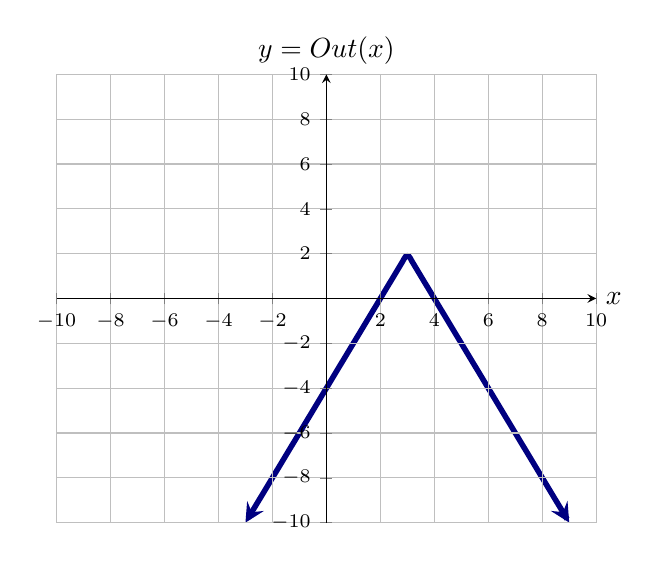
\begin{tikzpicture}
  \begin{axis}[
            domain=-10:10, ymax=10, xmax=10, ymin=-10, xmin=-10,
            axis lines =center, xlabel=$x$, ylabel={$y=Out(x)$}, grid = major,
            ytick={-10,-8,-6,-4,-2,2,4,6,8,10},
            xtick={-10,-8,-6,-4,-2,2,4,6,8,10},
            yticklabels={$-10$,$-8$,$-6$,$-4$,$-2$,$2$,$4$,$6$,$8$,$10$}, 
            xticklabels={$-10$,$-8$,$-6$,$-4$,$-2$,$2$,$4$,$6$,$8$,$10$},
            ticklabel style={font=\scriptsize},
            every axis y label/.style={at=(current axis.above origin),anchor=south},
            every axis x label/.style={at=(current axis.right of origin),anchor=west},
            axis on top
          ]
          
          %\addplot [line width=2, penColor2, smooth,samples=100,domain=(-6:2)] {-2*x-3};
      \addplot [line width=2, penColor, smooth,samples=100,domain=(-3:9),<->] {-2*abs(x-3)+2};

          %\addplot[color=penColor,fill=penColor2,only marks,mark=*] coordinates{(-6,9)};
          %\addplot[color=penColor,fill=penColor2,only marks,mark=*] coordinates{(2,-7)};



           

  \end{axis}
\end{tikzpicture}
\end{image}
The natural domain of $Out$ is $\mathbb{R}$. \\

If we think of moving through the domain from $-\infty$ to $\infty$, then the graph illustrates that $Out$ will increase on $(-\infty, 3]$ and decrease on $[3, \infty)$.  The function $Out$ has a maximum value of $\answer{2}$, which occurs at $\answer{3}$. \\


However, the output from $In$ is not $\mathbb{R}$, so we will not get the full output of $Out$. In addition, the output of $In$ will oscillate, which means the input values coming into $Out$ will osciallate.  This will make the output of $Out$ oscillate. \\






Graph of $z = In(t) = 2 \sin(t)+2$





\begin{image}
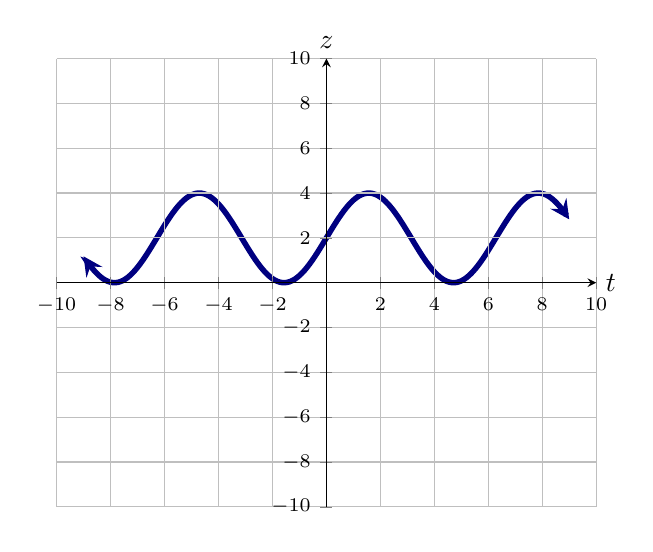
\begin{tikzpicture}
  \begin{axis}[
            domain=-10:10, ymax=10, xmax=10, ymin=-10, xmin=-10,
            axis lines =center, xlabel=$t$, ylabel=$z$, grid = major,
            ytick={-10,-8,-6,-4,-2,2,4,6,8,10},
            xtick={-10,-8,-6,-4,-2,2,4,6,8,10},
            yticklabels={$-10$,$-8$,$-6$,$-4$,$-2$,$2$,$4$,$6$,$8$,$10$}, 
            xticklabels={$-10$,$-8$,$-6$,$-4$,$-2$,$2$,$4$,$6$,$8$,$10$},
            ticklabel style={font=\scriptsize},
            every axis y label/.style={at=(current axis.above origin),anchor=south},
            every axis x label/.style={at=(current axis.right of origin),anchor=west},
            axis on top
          ]
          
          %\addplot [line width=2, penColor2, smooth,samples=100,domain=(-6:2)] {-2*x-3};
      \addplot [line width=2, penColor, smooth,samples=100,domain=(-9:9),<->] {2*sin(deg(x))+2};

          %\addplot[color=penColor,fill=penColor2,only marks,mark=*] coordinates{(-6,9)};
          %\addplot[color=penColor,fill=penColor2,only marks,mark=*] coordinates{(2,-7)};



           

  \end{axis}
\end{tikzpicture}
\end{image}




The input into $In(t)$ is the whole real line.  We naturally think of moving left to right, from $-\infty$ to $\infty$.  As we do this, the outputs from $In(t)$ oscillate between $0$ and $\answer{4}$.  Therefore, the inputs into $Out(x)$ oscillate back and forth inside the interval $\left[ \answer{0}, \answer{4} \right]$.





The output of $In(x)$ keeps going back and forth across the interval $[0,4]$. 

This becomes the input into $Out$.

Therefore, the input into $Out(x)$ keep going back and forth across the interval $[0,4]$. 








\begin{image}
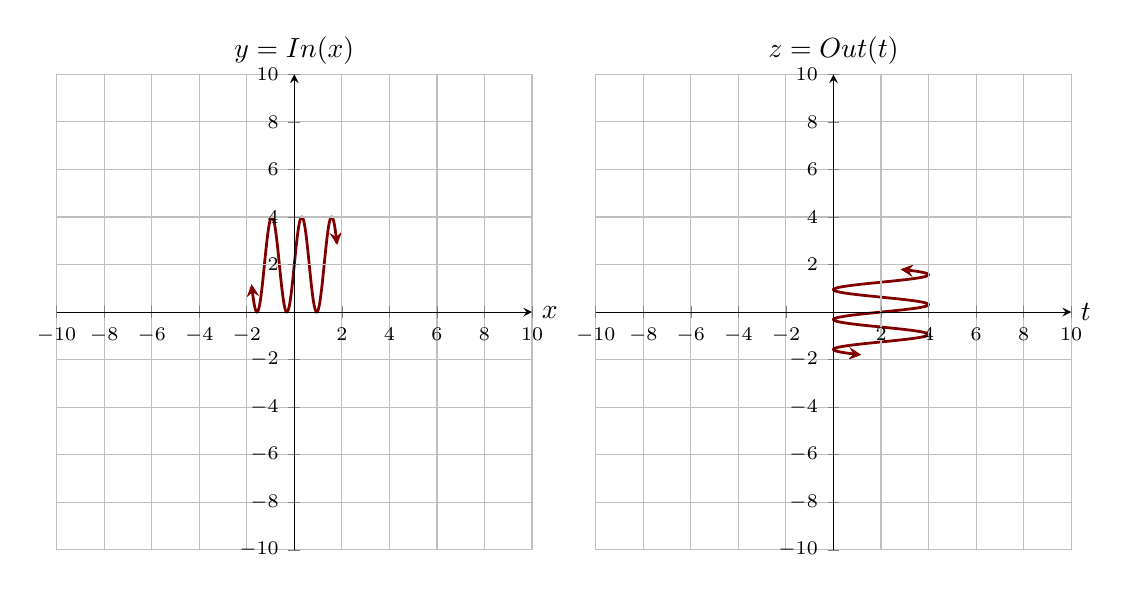
\begin{tikzpicture}
    \begin{axis}[name = sinax, domain=-10:10, ymax=10, xmax=10, ymin=-10, xmin=-10, width=3in, height=3in,
                  axis lines =center, xlabel=$x$, ylabel={$y=In(x)$}, grid = major,
                  ytick={-10,-8,-6,-4,-2,2,4,6,8,10},
                  xtick={-10,-8,-6,-4,-2,2,4,6,8,10},
                  yticklabels={$-10$,$-8$,$-6$,$-4$,$-2$,$2$,$4$,$6$,$8$,$10$}, 
                  xticklabels={$-10$,$-8$,$-6$,$-4$,$-2$,$2$,$4$,$6$,$8$,$10$},
                  ticklabel style={font=\scriptsize},
                  every axis y label/.style={at=(current axis.above origin),anchor=south},
                  every axis x label/.style={at=(current axis.right of origin),anchor=west},
                  axis on top]
         \addplot [line width=1, penColor2, smooth,samples=300,domain=(-9:9),<->] ({0.2*x}, {2*sin(deg(x))+2});

    \end{axis}
    \begin{axis}[at={(sinax.outer east)},anchor=outer west, domain=-10:10, ymax=10, xmax=10, ymin=-10, xmin=-10, 
                  width=3in, height=3in,
                  axis lines =center, xlabel=$t$, ylabel={$z=Out(t)$}, grid = major,
                  ytick={-10,-8,-6,-4,-2,2,4,6,8,10},
                  xtick={-10,-8,-6,-4,-2,2,4,6,8,10},
                  yticklabels={$-10$,$-8$,$-6$,$-4$,$-2$,$2$,$4$,$6$,$8$,$10$}, 
                  xticklabels={$-10$,$-8$,$-6$,$-4$,$-2$,$2$,$4$,$6$,$8$,$10$},
                  ticklabel style={font=\scriptsize},
                  every axis y label/.style={at=(current axis.above origin),anchor=south},
                  every axis x label/.style={at=(current axis.right of origin),anchor=west},
                  axis on top]
         \addplot [line width=1, penColor2, smooth,samples=300,domain=(-9:9),<->] ({2*sin(deg(x))+2},{0.2*x});

    \end{axis}


\end{tikzpicture}
\end{image}



What part of the graph of $Out$ does this oscillation run across?



\begin{image}
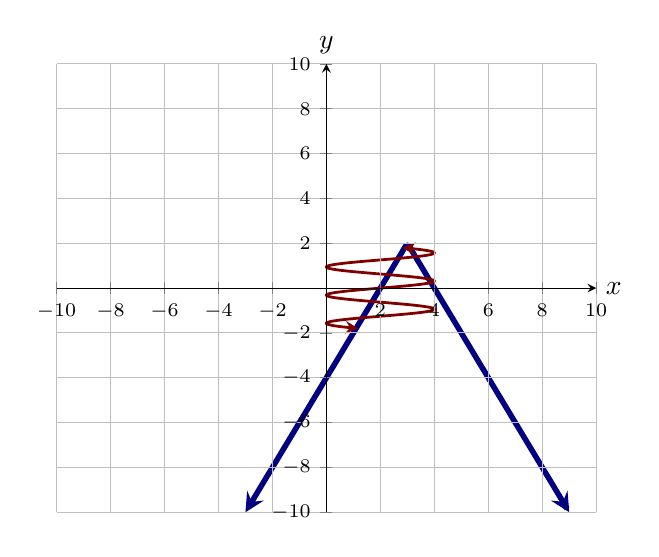
\begin{tikzpicture}
  \begin{axis}[
            domain=-10:10, ymax=10, xmax=10, ymin=-10, xmin=-10,
            axis lines =center, xlabel=$x$, ylabel=$y$, grid = major,
            ytick={-10,-8,-6,-4,-2,2,4,6,8,10},
            xtick={-10,-8,-6,-4,-2,2,4,6,8,10},
            yticklabels={$-10$,$-8$,$-6$,$-4$,$-2$,$2$,$4$,$6$,$8$,$10$}, 
            xticklabels={$-10$,$-8$,$-6$,$-4$,$-2$,$2$,$4$,$6$,$8$,$10$},
            ticklabel style={font=\scriptsize},
            every axis y label/.style={at=(current axis.above origin),anchor=south},
            every axis x label/.style={at=(current axis.right of origin),anchor=west},
            axis on top
          ]
          
          %\addplot [line width=2, penColor2, smooth,samples=100,domain=(-6:2)] {-2*x-3};
      \addplot [line width=2, penColor, smooth,samples=100,domain=(-3:9),<->] {-2*abs(x-3)+2};

      \addplot [line width=1, penColor2, smooth,samples=300,domain=(-9:9),<->] ({2*sin(deg(x))+2},{0.2*x});

          %\addplot[color=penColor,fill=penColor2,only marks,mark=*] coordinates{(-6,9)};
          %\addplot[color=penColor,fill=penColor2,only marks,mark=*] coordinates{(2,-7)};



           

  \end{axis}
\end{tikzpicture}
\end{image}

The only part of the graph of $Out$ that is used is on the interval $[0, 4]$.






\begin{image}
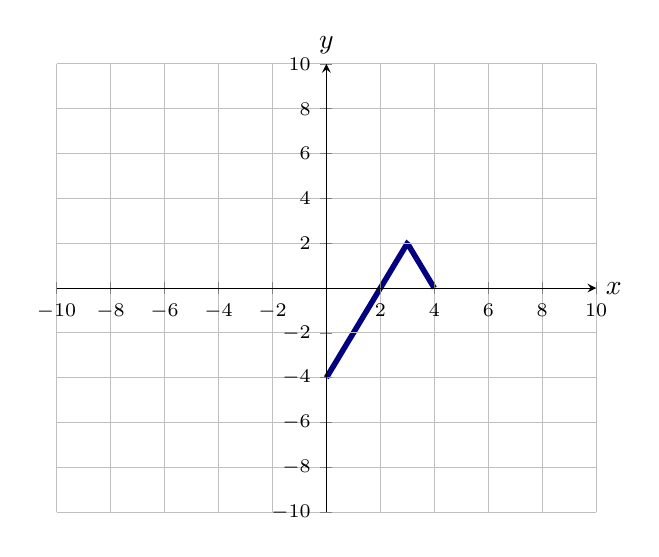
\begin{tikzpicture}
  \begin{axis}[
            domain=-10:10, ymax=10, xmax=10, ymin=-10, xmin=-10,
            axis lines =center, xlabel=$x$, ylabel=$y$, grid = major,
            ytick={-10,-8,-6,-4,-2,2,4,6,8,10},
            xtick={-10,-8,-6,-4,-2,2,4,6,8,10},
            yticklabels={$-10$,$-8$,$-6$,$-4$,$-2$,$2$,$4$,$6$,$8$,$10$}, 
            xticklabels={$-10$,$-8$,$-6$,$-4$,$-2$,$2$,$4$,$6$,$8$,$10$},
            ticklabel style={font=\scriptsize},
            every axis y label/.style={at=(current axis.above origin),anchor=south},
            every axis x label/.style={at=(current axis.right of origin),anchor=west},
            axis on top
          ]
          
          %\addplot [line width=2, penColor2, smooth,samples=100,domain=(-6:2)] {-2*x-3};
      \addplot [line width=2, penColor, smooth,samples=100,domain=(0:4)] {-2*abs(x-3)+2};

  \end{axis}
\end{tikzpicture}
\end{image}






Therefore, that part of the graph of $Out$ just keeps repeating back and forth. 







\begin{image}
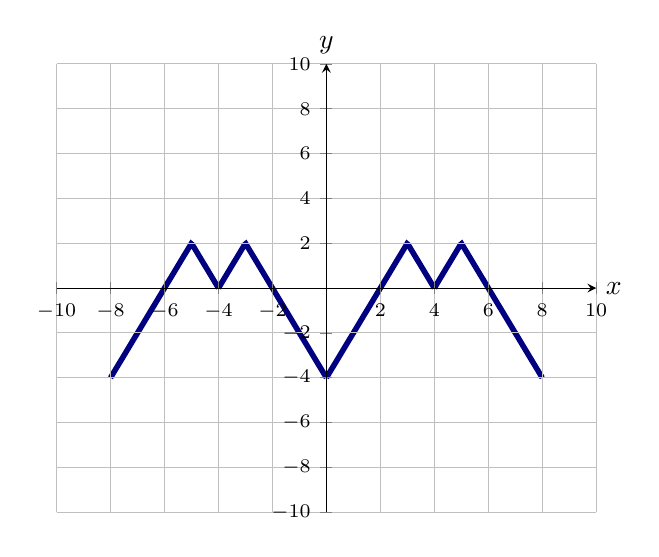
\begin{tikzpicture}
  \begin{axis}[
            domain=-10:10, ymax=10, xmax=10, ymin=-10, xmin=-10,
            axis lines =center, xlabel=$x$, ylabel=$y$, grid = major,
            ytick={-10,-8,-6,-4,-2,2,4,6,8,10},
            xtick={-10,-8,-6,-4,-2,2,4,6,8,10},
            yticklabels={$-10$,$-8$,$-6$,$-4$,$-2$,$2$,$4$,$6$,$8$,$10$}, 
            xticklabels={$-10$,$-8$,$-6$,$-4$,$-2$,$2$,$4$,$6$,$8$,$10$},
            ticklabel style={font=\scriptsize},
            every axis y label/.style={at=(current axis.above origin),anchor=south},
            every axis x label/.style={at=(current axis.right of origin),anchor=west},
            axis on top
          ]
          
          %\addplot [line width=2, penColor2, smooth,samples=100,domain=(-6:2)] {-2*x-3};
      \addplot [line width=2, penColor, smooth,samples=100,domain=(-8:-4)] {-2*abs(x+8-3)+2};
      \addplot [line width=2, penColor, smooth,samples=100,domain=(-4:0)] {-2*abs(x+3)+2};
      \addplot [line width=2, penColor, smooth,samples=100,domain=(0:4)] {-2*abs(x-3)+2};
      \addplot [line width=2, penColor, smooth,samples=100,domain=(4:8)] {-2*abs(x-8+3)+2};

  \end{axis}
\end{tikzpicture}
\end{image}


Except, the ``$+2$'' in $In(t) = 2 \sin(t) + 2$ will become the input for $Out$.  This will cause a horizontal shift for $Out$. 






The smooth rounding of the sine curve will round out the corners of the absolute value graph and the $2\pi$ period of $\sin(t)$ will force the same period for the composition.







\begin{image}
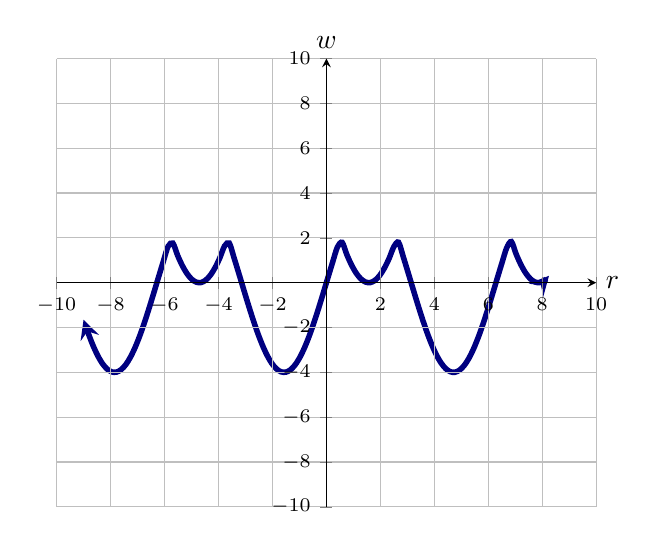
\begin{tikzpicture}
  \begin{axis}[
            domain=-10:10, ymax=10, xmax=10, ymin=-10, xmin=-10,
            axis lines =center, xlabel=$r$, ylabel=$w$, grid = major,
            ytick={-10,-8,-6,-4,-2,2,4,6,8,10},
            xtick={-10,-8,-6,-4,-2,2,4,6,8,10},
            yticklabels={$-10$,$-8$,$-6$,$-4$,$-2$,$2$,$4$,$6$,$8$,$10$}, 
            xticklabels={$-10$,$-8$,$-6$,$-4$,$-2$,$2$,$4$,$6$,$8$,$10$},
            ticklabel style={font=\scriptsize},
            every axis y label/.style={at=(current axis.above origin),anchor=south},
            every axis x label/.style={at=(current axis.right of origin),anchor=west},
            axis on top
          ]
          
          %\addplot [line width=2, penColor2, smooth,samples=100,domain=(-6:2)] {-2*x-3};
      \addplot [line width=2, penColor, smooth,samples=100,domain=(-9:8.25),<->] {-2*abs((2*sin(deg(x))+2)-3)+2};

      %\addplot [line width=1, penColor2, smooth,samples=300,domain=(-9:9),<->] ({2*sin(deg(x))+2},{0.2*x});

          %\addplot[color=penColor,fill=penColor2,only marks,mark=*] coordinates{(-6,9)};
          %\addplot[color=penColor,fill=penColor2,only marks,mark=*] coordinates{(2,-7)};



           

  \end{axis}
\end{tikzpicture}
\end{image}




\end{explanation}

\end{example}



\textbf{\textcolor{red!70!black}{Notice:}} 



We are repeating the piece of $Out$ on the interval $[0,4]$.  \\



$\blacktriangleright$ The minimum value of $Out$ occurs at $0$.  When does the oputput of $In$ equal $0$?



$In(t) = 2 \sin(t)+2 = 0$ when $sin(t) = -1$, which is when $t = -\frac{\pi}{2} + 2k\pi$ where $k \in \mathbb{N}$. We can see this as the lower valleys in the graph of the composition.





$\blacktriangleright$ The maximum value of $Out$ occurs at $3$.  When does the oputput of $In$ equal $3$?



$In(t) = 2 \sin(t)+2 = 3$ when $sin(t) = \frac{1}{2}$, which is when $t = \frac{\pi}{6} + 2k\pi$ and $t = \frac{5\pi}{6} + 2k\pi$ where $k \in \mathbb{N}$. We can see this as the two peaks in the graph of the composition.

















Graphically, we have to keep our eyes on several things at once.  We watch the original input into $In$, then we watch the output of $In$ and picture that as the new input into $Out$, then we watch the output coming from $Out$.
































\begin{example} Composition


\begin{itemize}
\item Let $K(u) = \frac{u}{u-1}$ with its natural or implied domain: $(-\infty, 1) \cup (1, \infty)$. \\

\item Let $T(w) = w^2 + 5w + 7$ with its natural or implied domain: \textbf{$\mathbb{R}$}.
\end{itemize}


Form the composition $K \circ T$.

\[        (K \circ T)(w) =     \frac{w^2 + 5w + 7}{(w^2 + 5w + 7)-1}   =    \frac{w^2 + 5w + 7}{w^2 + 5w + 6}  \]


$K$ can accept any number, except $1$.  Therefore we need to find out when $T = 1$ and take out the domain numbers where $1$ occurs.



\begin{align*}
T(w) & = 1   \\
w^2 + 5w + 7 & = 1 \\
w^2 + 5w + 6 & = 0   \\
(w+2)\left( \answer{w+3} \right) & = 0
\end{align*}


We need to remove $-2$ and $\answer{-3}$ from the domain of $K \circ T$, because $T(-2)=1$ and $T(-3)=1$ and $1$ cannot be an input into $K$.


The domain for $K \circ T$ is $(-\infty, -3) \cup (-3, -2) \cup (-2, \infty)$




\[        (K \circ T)(w)  =  K(T(w))  = \frac{w^2 + 5w + 7}{w^2 + 5w + 6}  =    \frac{w^2 + 5w + 7}{(w+2)(w+3)} \]










The composition is a function. \\


This is a good reminder that a formula is not a function. There are always domain considerations.  In the case of a composition, we need to restrict the domain of the inner function to avoid inner function values that are not in the domain of the outer function.










\end{example}










\begin{example} Composition



\begin{itemize}
\item Let $g(x) = \frac{x-3}{x+1}$ with its natural or implied domain: $(-\infty, -1) \cup (-1. \infty)$. \\

\item Let $H(t) = \frac{t+3}{1-t}$ with its natural or implied domain: $(-\infty, 1) \cup (1. \infty)$.
\end{itemize}



\[
(g \circ H)(y) = g(H(y)) = \frac{\left( \frac{y+3}{1-y} \right) - 3}{\left(  \frac{y+3}{1-y}\right) + 1} = \frac{y+3-3(1-y)}{y+3+(1-y)} = \frac{4y}{4} = y
\]



$g$ and $H$ are inverse functions.




\end{example}

Of course, that isn't the whole story.  As we said earlier, formulas are not functions. \\

$(g \circ H)(r) = r$ and so $g \circ H = Id$, the identity function.  But remember our caveat.  There are always domain issues.  In this case $(g \circ H)(r) = r$ for almost all of the real numbers.

We know that, 


\[
(g \circ H)(r) = \frac{\left( \frac{r+3}{1-r} \right) - 3}{\left(  \frac{r+3}{1-r}\right) + 1} 
\]


This is equivalent to $r$ for almost all real numbers.


In this case, $(g \circ H)(r) = g(H(r))$, which means that $r \ne 1$, since $1$ is not in the domain of $H$.  Secondly, $-1$ is not in the domain of $g$.  We also cannot have values of $r$ that make $H(r) = -1$.




\[
H(r) = \frac{r+3}{1-r} = -1
\]

\[
r + 3 = -(1-r) = -1 + r
\]


\[
3 = -1
\]


There are no such real numbers.


Wait.  There is more to this story. We would like the other way as well: $(H \circ g)(z) = z$ and so $H \circ g = Id$.


Thus, $z \ne -1$.  We must also avoid $g(z) = 1$, because $1$ is not in the domain of $H$.



\[
g(z) = \frac{z-3}{z+1} = 1
\]

\[
z - 3 = z + 1 
\]


\[
-3 = 1
\]


There are no such real numbers.













$\blacktriangleright$ Therefore, $g$ and $H$ are inverse functions on $(-\infty, 1) \cup (-1, 1) \cup (1,\infty)$.




















\section*{The Other Half of the Story}


We would like our function arithmetic to mimic our arithmetic for numbers.  For numbers, the inverses are commutative.

\[
4 + (-4) = (-4) + 4 = 0
\]


\[
4 \cdot \frac{1}{4} = \frac{1}{4} \cdot 4 = 1
\]



In our example, we also want $(H \circ g)(z) = H(g(z)) = z$. It does.


\[
(H \circ g)(z) = \frac{\left( \frac{z-3}{z+1} \right) + 3}{1 - \left(  \frac{z-3}{z+1}\right)} = \frac{z-3 + 3(z+1)}{z+1-(z-3)} = \frac{4z}{4} = z
\]


In this case, we cannot have $z = -1$






$\blacktriangleright$  Therefore, $g$ and $H$ are inverse functions on $(-\infty, -1) \cup (-1, 1) \cup (1, \infty)$.












































\subsection*{Algebraically}










\textbf{\textcolor{purple!85!blue}{Algebraically, we just replace.}}

















\section*{Algebraically}







Let $Out(x) = 3x^3 + \sin(4x) - \frac{3}{2-x}$ with its natural or implied domain. \\
Let $In(t) = \frac{5t-7}{t^2-8}$ with its natural or implied domain. \\



Algebraically, composition is accomplished by replacing all occurences of the variable with the entire formula for the other function.




\[
(Out \circ In)(k) = Out(In(k)) = 3 \left( \frac{5k-7}{k^2-8} \right)^3 + \sin(4 \frac{5k-7}{k^2-8}) - \frac{3}{2-\frac{5t-7}{k^2-8}}
\]





Obviously, parentheses are vital here.





\[
(Out \circ In)(k) = Out(In(k)) = 3 \left( \frac{5k-7}{k^2-8} \right)^3 + \sin\left( 4 \left( \frac{5k-7}{k^2-8} \right) \right) - \frac{3}{2 - \left( \frac{5k-7}{k^2-8} \right)}
\]






We can always make two compositions from two functions.




\[
(In \circ Out)(u) = In(Out(u)) = \frac{5 \left( 3u^3 + \sin(4u) - \frac{3}{2-u} \right)-7}{\left( 3u^3 + \sin(4u) - \frac{3}{2-u} \right)^2-8}
\]





\begin{example} Composition 



Let $f(x) = 5x^2 - 4x + 2$ with its natural or implied domain. \\
Let $g(t) = \frac{3}{6-t}$ with its natural or implied domain. \\



\[
(f \circ g)(y) = f(g(y)) = 5 \left( \answer{\frac{3}{6-y}} \right)^2 - 4 \left( \answer{\frac{3}{6-y}} \right) + 2
\]





\[
(g \circ f)(w) = g(f(w)) = \frac{3}{6 - \left( \answer{5w^2 - 4w + 2} \right)}
\]



\end{example}










\begin{example} Composition 



Let $f(x) = 3x^2 - x + 5$ with its natural or implied domain. \\
Let $g(t) = \frac{4}{7-t}$ with its natural or implied domain. \\



Thinking about $(g \circ f)(w) = g(f(w))$... \\

There are two numbers where $f(x) = 7$.  One of them is $1$, the other is $\answer{\frac{-2}{3}}$.






\[
(g \circ f)(w) = g(f(w)) = \frac{4}{7 - (5w^2 - 4w + 2)}
\]



In the $g \circ f$ composition, $f$ is no longer allowed to equal $\answer{7}$.

Select all real numbers which cannot be in the domain of $g \circ f$.

\begin{selectAll}
\choice{$7$}
\choice{$0$}
\choice[correct]{$1$}
\choice{$\frac{2}{3}$}
\choice{$-1$}
\choice[correct]{$\frac{-2}{3}$}
\end{selectAll}


\end{example}

























\subsection*{Decompose}



















\begin{example}


Let $H(d)$ and $M(p)$ be two functions and $H \circ M$ be their composition.


Suppose $M(p) = 3 p - 5$ \\

Suppose $(H \circ M)(k) = 5 k + 1$


Find $H(d)$.



\begin{explanation}




$(H \circ M)(k) = H(M(k)) = H(3 k - 5)$  \\



$H$ is going to do something to $3 k - 5$ and produce $5 k + 1$. \\




These are both linear functions, therefore $H(d)$ should be a linear function.


First $H$ should multiply $3 k - 5$ by $\answer{\frac{5}{3}}$ to produce a $5k$.


\[    \frac{5}{3} (3 k - 5) = 5k - \frac{25}{3}   \]



Now, we need $-\frac{25}{3}$ to become $1$.  $H$ should add $\answer{\frac{28}{3}}$.

\[  H(d) =    \frac{5}{3} d +     \frac{28}{3} \]



$\blacktriangleright$ Check: 


\[    (H \circ M)(k) = H(M(k)) = H(3 k - 5) =    \frac{5}{3} (3 k - 5) +     \frac{28}{3}  = 5k - \frac{25}{3}  + \frac{28}{3}  = 5k + \frac{3}{3}  = 5k + 1\]





\end{explanation}

\end{example}













\begin{example}


Let $H(d)$ and $M(p)$ be two functions and $H \circ M$ be their composition.


Suppose $H(d) = 3 d - 5$ \\

Suppose $(H \circ M)(k) = 5 k + 1$


Find $M(p)$.



\begin{explanation}




$(H \circ M)(k) = H(M(k)) = 3 M(k) - 5 $  \\




These are both linear functions, therefore $M(k)$ should be a linear function.


$M$ is going to be multiplied by $3$, therefore $M$ should start with $M(p) = \answer{\frac{5}{3}}p$. That way, when it is multiplied by $3$, we will get $5p$.




Now, we need $3$ times something to be $1$.  $M$ should add $\answer{\frac{1}{3}}$.

\[  M(p) =    \frac{5}{3} p +     \frac{1}{3} \]



$\blacktriangleright$ Check: 


\[    (H \circ M)(k) = H(M(k)) = 3 \left( \frac{5}{3} k + \frac{1}{3} \right) - 5 =    5 k + 1 -5 = 5 k -4    \]




\end{explanation} 

\end{example}










\begin{example}


Let $f(x)$ and $g(w)$ be two functions and $f \circ g$ be their composition.


Suppose $g(w) = 3w + 1$ \\

Suppose $(f \circ g)(t) = \frac{2t}{t-1}$


Find $f(x)$.



\begin{explanation}




$(f \circ g)(t) =  f(g(t)) =  \frac{2t}{t-1}$ \\



The composition has two occurrences of the variable.  $g$ has one occurrence and when it is put into $f$ the resulting formula has two occurrences.  It seems reasonable to guess that $f$ has two occurences of its variable - one in a numerator and one in a denominator.  $3t + 1$ will replace each in the composition.

So, let's start constructing. \\


$\blacktriangleright$  \textbf{\textcolor{blue!55!black}{Guess \#1)}}   \\

Let's start with two occurences of $x$, one in the numerator and one in the denominator.

\[      f(x) = \frac{x}{x}       \]


this makes the composition look like

\[   f(g(t)) =      \frac{3t + 1}{3t + 1}       \]



We need the coefficients of $t$ to be $2$ in the numerator and $1$ in the denominator.

$\blacktriangleright$  \textbf{\textcolor{blue!55!black}{Guess \#2)}}   \\

\[   f(g(t)) =      \frac{\answer{\frac{2}{3}}(3t + 1)}{\frac{1}{3}(3t + 1)}       \]

That gives


\[   f(g(t)) =      \frac{2t + \frac{2}{3}}{t + \frac{1}{3}}       \]



Now, we need constant terms of $0$ in the numerator and $-1$ in the denominator.  Subtract $\answer{\frac{2}{3}}$ from the numerator. Subtract $\answer{\frac{4}{3}}$ from the denominator. \\

$\blacktriangleright$  \textbf{\textcolor{blue!55!black}{Guess \#3)}}   \\


\[   f(g(t)) =      \frac{\frac{2}{3}(3t + 1) - \frac{2}{3}}{\frac{1}{3}(3t + 1) - \frac{4}{3}}       \]

That tells us what $f$ needs to do.




\[   f(x) =      \frac{\frac{2}{3}x - \frac{2}{3}}{\frac{1}{3}x - \frac{4}{3}}       \]



\end{explanation}

\end{example}























\begin{example}


Let $H(x)$ and $B(w)$ be two functions and $B \circ H$ be their composition.


Suppose $B(w) = 3w + 1$ \\

Suppose $(B \circ H)(t) = \frac{2t}{t-1}$


Find $H(x)$.



\begin{explanation}




$(B \circ H)(t) =  B(H(t)) = 3 H(t) + 1$ \\


We want this to equal $\frac{2t}{t-1}$.




\[
3 H(t) + 1 = \frac{2t}{t-1}
\]


We can solve for $H(t)$.



\[
3 H(t) + 1 = \frac{2t}{t-1}
\]

\[
3 H(t) = \frac{2t}{t-1} - 1 = \frac{\answer{t+1}}{t-1}
\]

\[
H(t)  = \answer{\frac{t+1}{3(t-1)}}
\]



Check:

\[
(B \circ H)(t) =  B(H(t)) = 3 H(t) + 1 = 3 \left( \frac{t+1}{3(t-1)} \right) + 1 = \frac{3(t+1) + 3(t-1)}{3(t-1)} 
\]


\[
 = \frac{(t+1) + (t-1)}{(t-1)}  = \frac{2t}{(t-1)}
\]



\end{explanation}

\end{example}

































\begin{center}
\textbf{\textcolor{green!50!black}{ooooo-=-=-=-ooOoo-=-=-=-ooooo}} \\

more examples can be found by following this link\\ \link[More Examples of Composition]{https://ximera.osu.edu/csccmathematics/precalculus1/precalculus1/composition/examples/exampleList}

\end{center}







\end{document}
